\documentclass{article}
\usepackage{graphicx}
\usepackage{float}
\usepackage[spanish]{babel}
\usepackage{hyperref}
\usepackage{csquotes}
\graphicspath{ {img/} }
\setlength{\parskip}{\baselineskip}

\title{Areas Recreativas - Sprint 2 \\[3ex] \small PAMN - Programación de Aplicaciónes Moviles Nativas}

\author{Chamil José Cruz Razeq}

\begin{document}
    \maketitle
    \thispagestyle{empty}
    \newpage

    \section{Introducción}
        Todos los informes sobre las tareas propuestas se encuentran disponibles en el
         siguiente repositorio de \href{https://github.com/chamilstudy/ulpgc_pamn_labs}{GitHub}
         y la aplicación se encuentra en \href{https://github.com/chamilstudy/pamn_proyecto_final}{GitHub}.

        Este documento recoge la información referente al segundo sprint del desarrollo de la
         aplicación de Areas Recreativas.
    
    \section{Historias de Usuario}

    Entre las historias de usuario planteadas, se han seleccionado para el segundo sprint:
    
    \begin{figure}[H]
        \centerline{\includegraphics[scale=0.4]{historias.png}}
        \caption{Historias de usuario}
        \label{fig:historias}
    \end{figure}

    Donde podemos establecer los siguientes objetivos:

    \begin{itemize}
        \item Desarrollo de pantalla y modelos para la vista de areas disponibles.
        \item Desarrollo de pantalla y modelo para vista de area seleccionada, sus características
            y formulacio de solicitud.
        \item Desarrollo de pantalla y modelo de solicitudes y formulario de eliminación.
        \item Desarrollo de pantalla y modelo de emergencias y redirección al método de contacto.
        \item Desarrollo de pantalla y modelo del perfil con boton de cierre de sesión.
    \end{itemize}

    \section{Estimación en tiempo de cada historia}

    Para cada uno de los objetivos anteriores podría dedicarse entre 4-7 horas, acumulando en el
     caso mas favorable unas 20 horas de desarrollo o en el mas desfavorable unas 35 horas.

    Adicionalmente, al tratarse del primer sprint, configurar el proyecto, crear directorios y
     ficheros, configurar el manifiesto y ficheros de build podría llevar unas 4 horas.

    \section{Reparto de tareas}

    Todas las tareas serán desarrolladas por el autor de este documento.

    \section{Muestra de desarrollo}

    \begin{figure}[H]
        \centerline{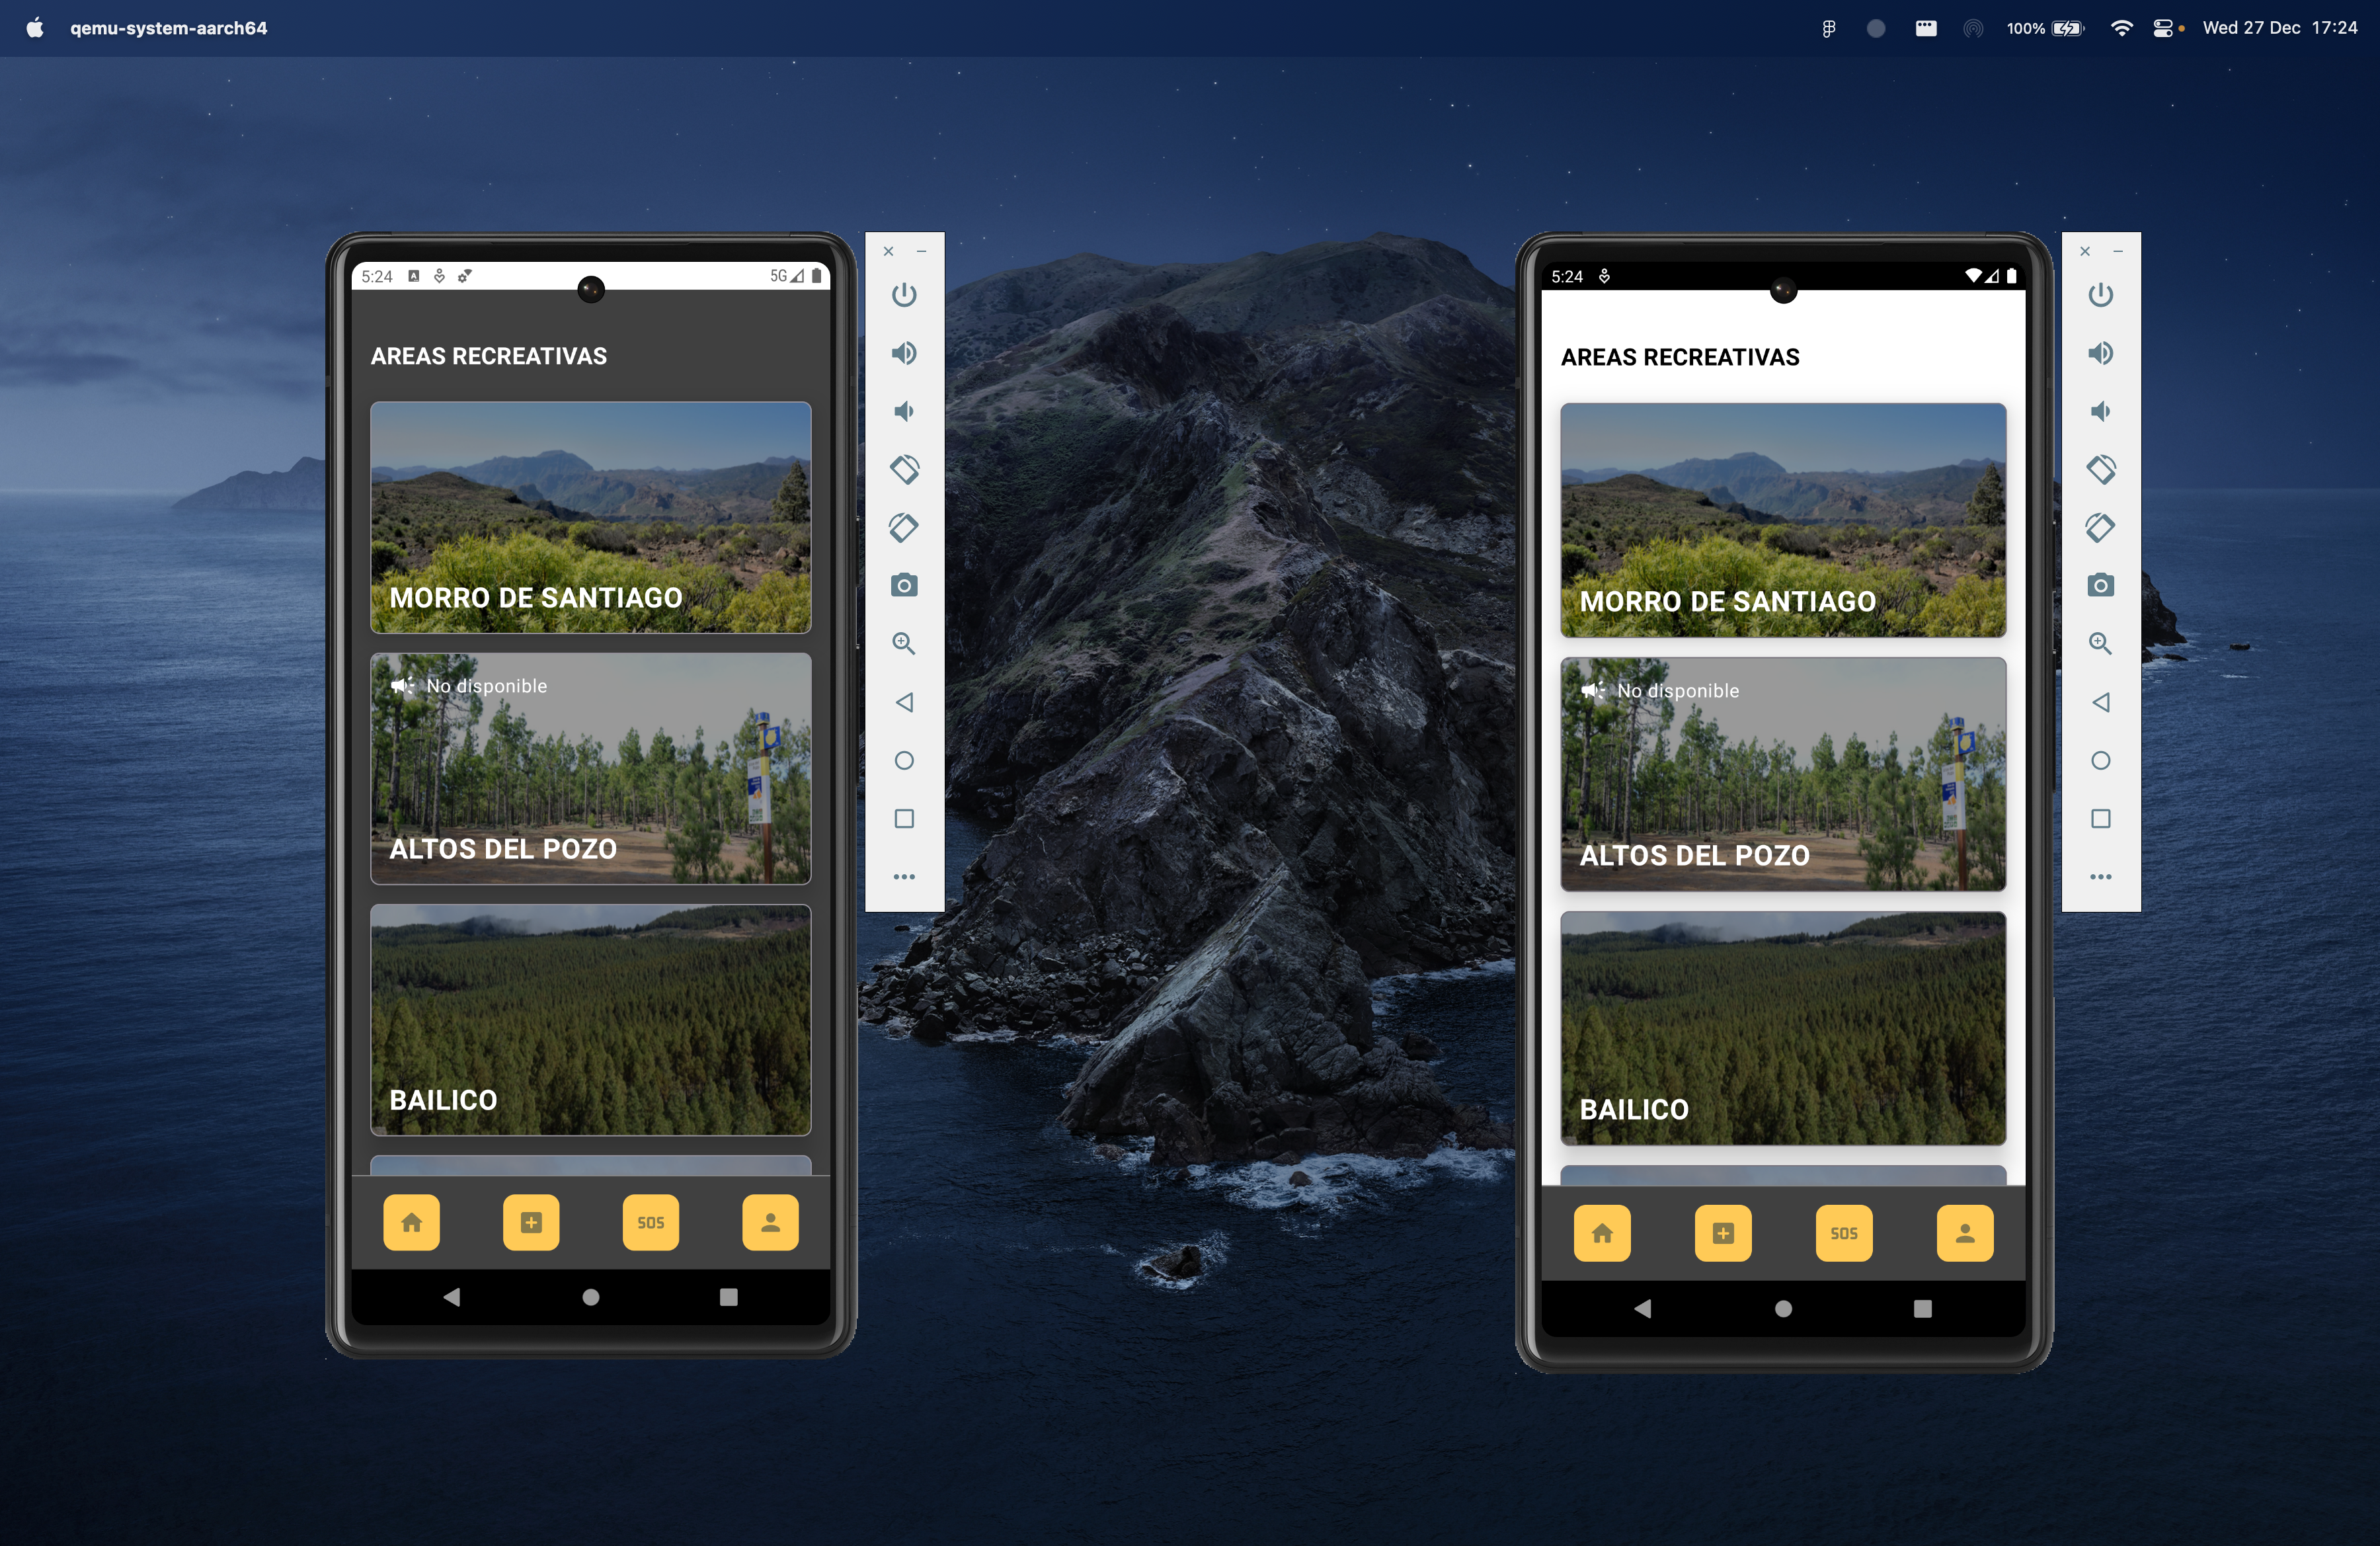
\includegraphics[scale=0.2]{home.png}}
        \caption{Pantalla principal}
        \label{fig:home}
    \end{figure}

    \begin{figure}[H]
        \centerline{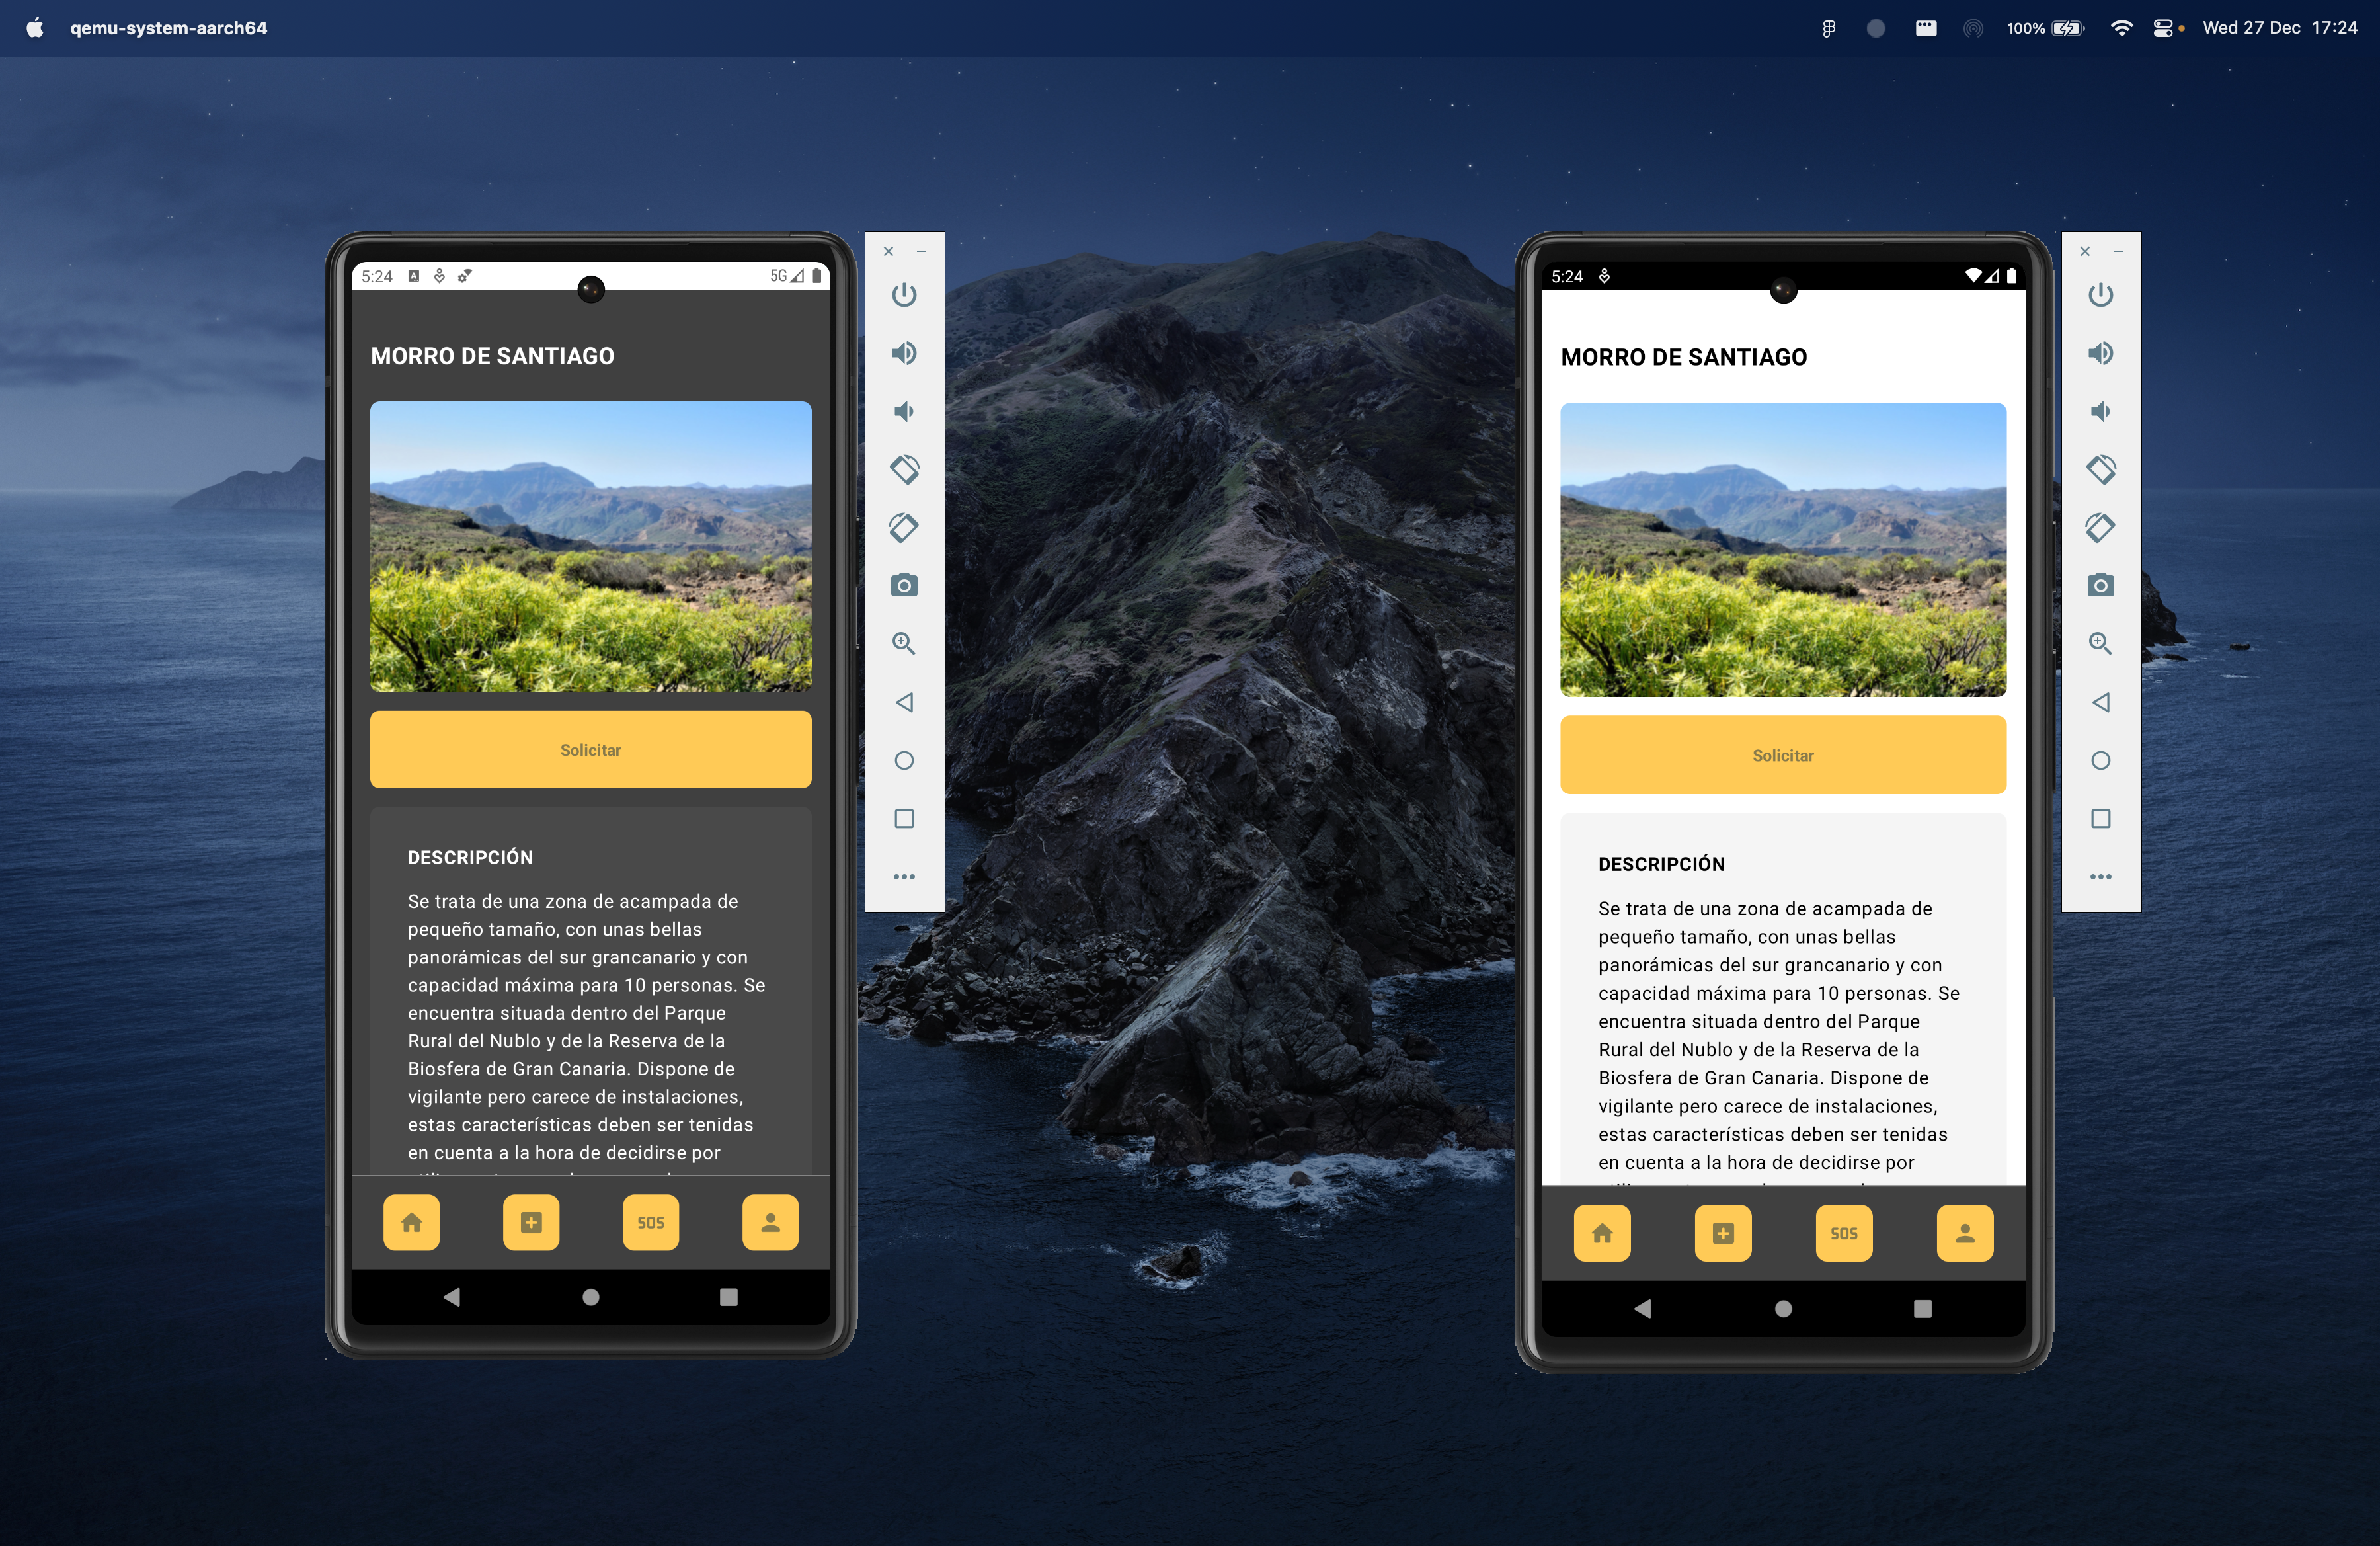
\includegraphics[scale=0.2]{area1.png}}
        \caption{Pantalla de area seleccionada}
        \label{fig:area1}
    \end{figure}

    \begin{figure}[H]
        \centerline{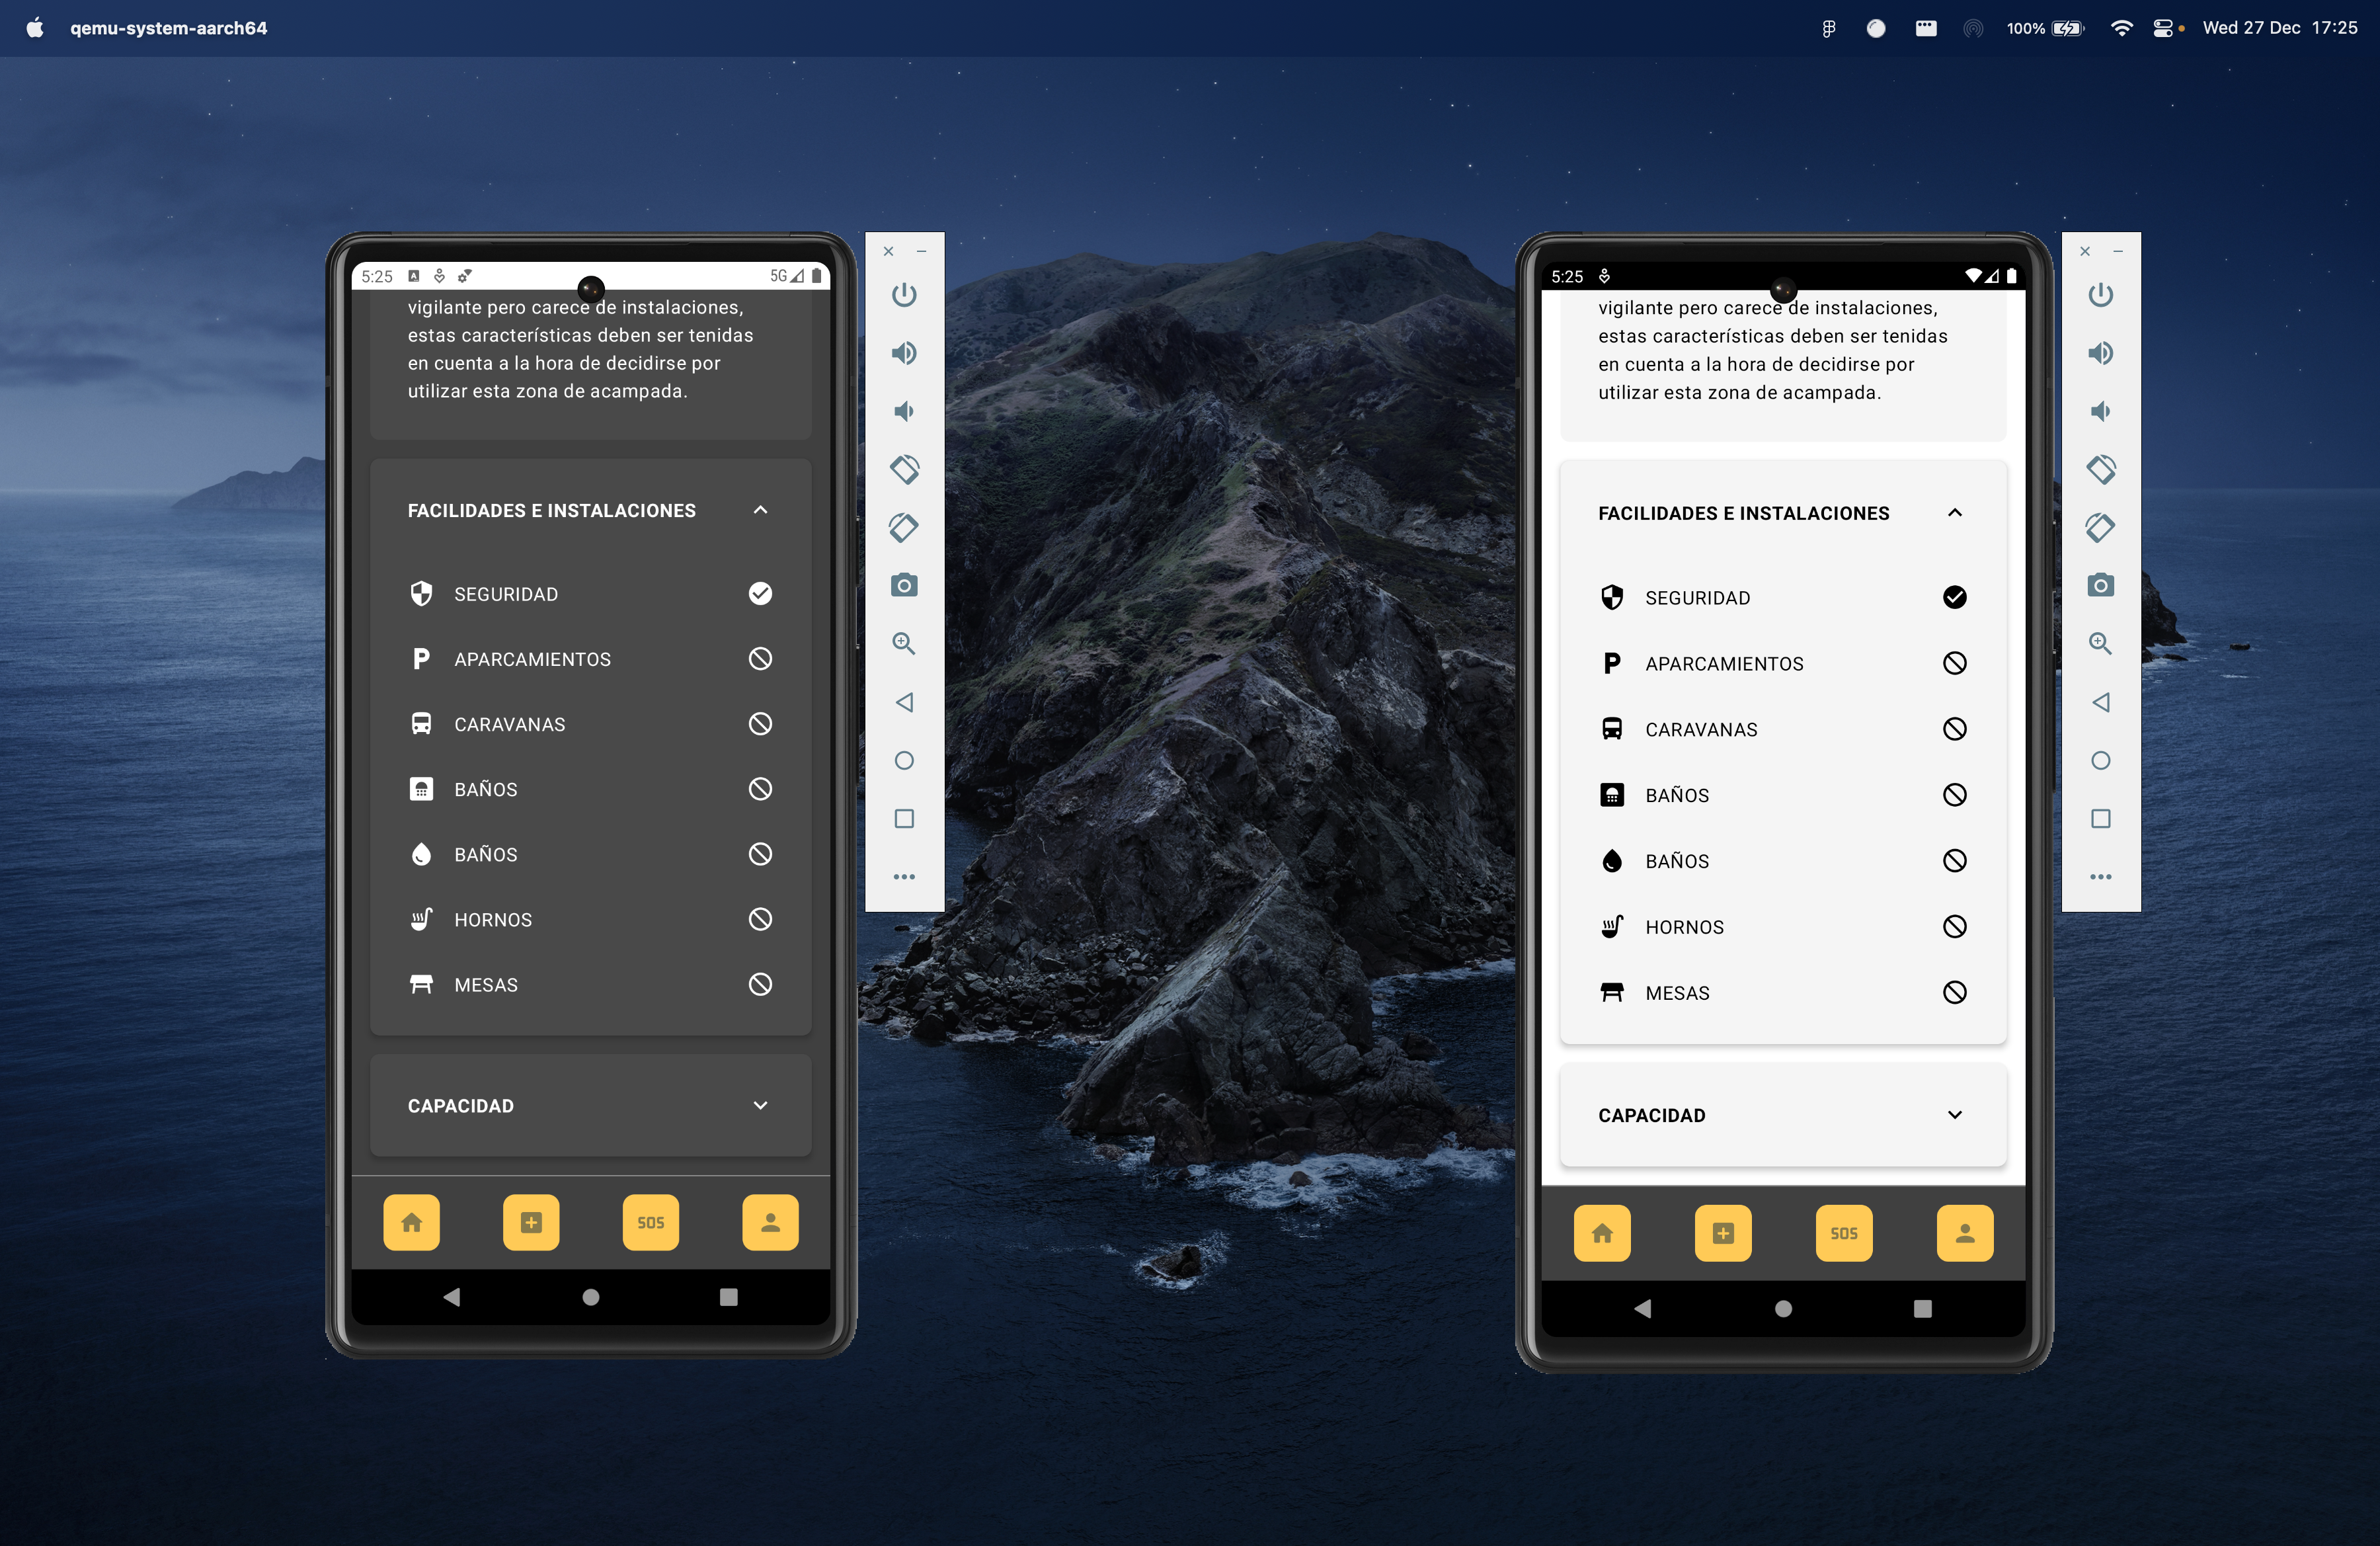
\includegraphics[scale=0.2]{area2.png}}
        \caption{Pantalla de area seleccionada con desplegable}
        \label{fig:area2}
    \end{figure}

    \begin{figure}[H]
        \centerline{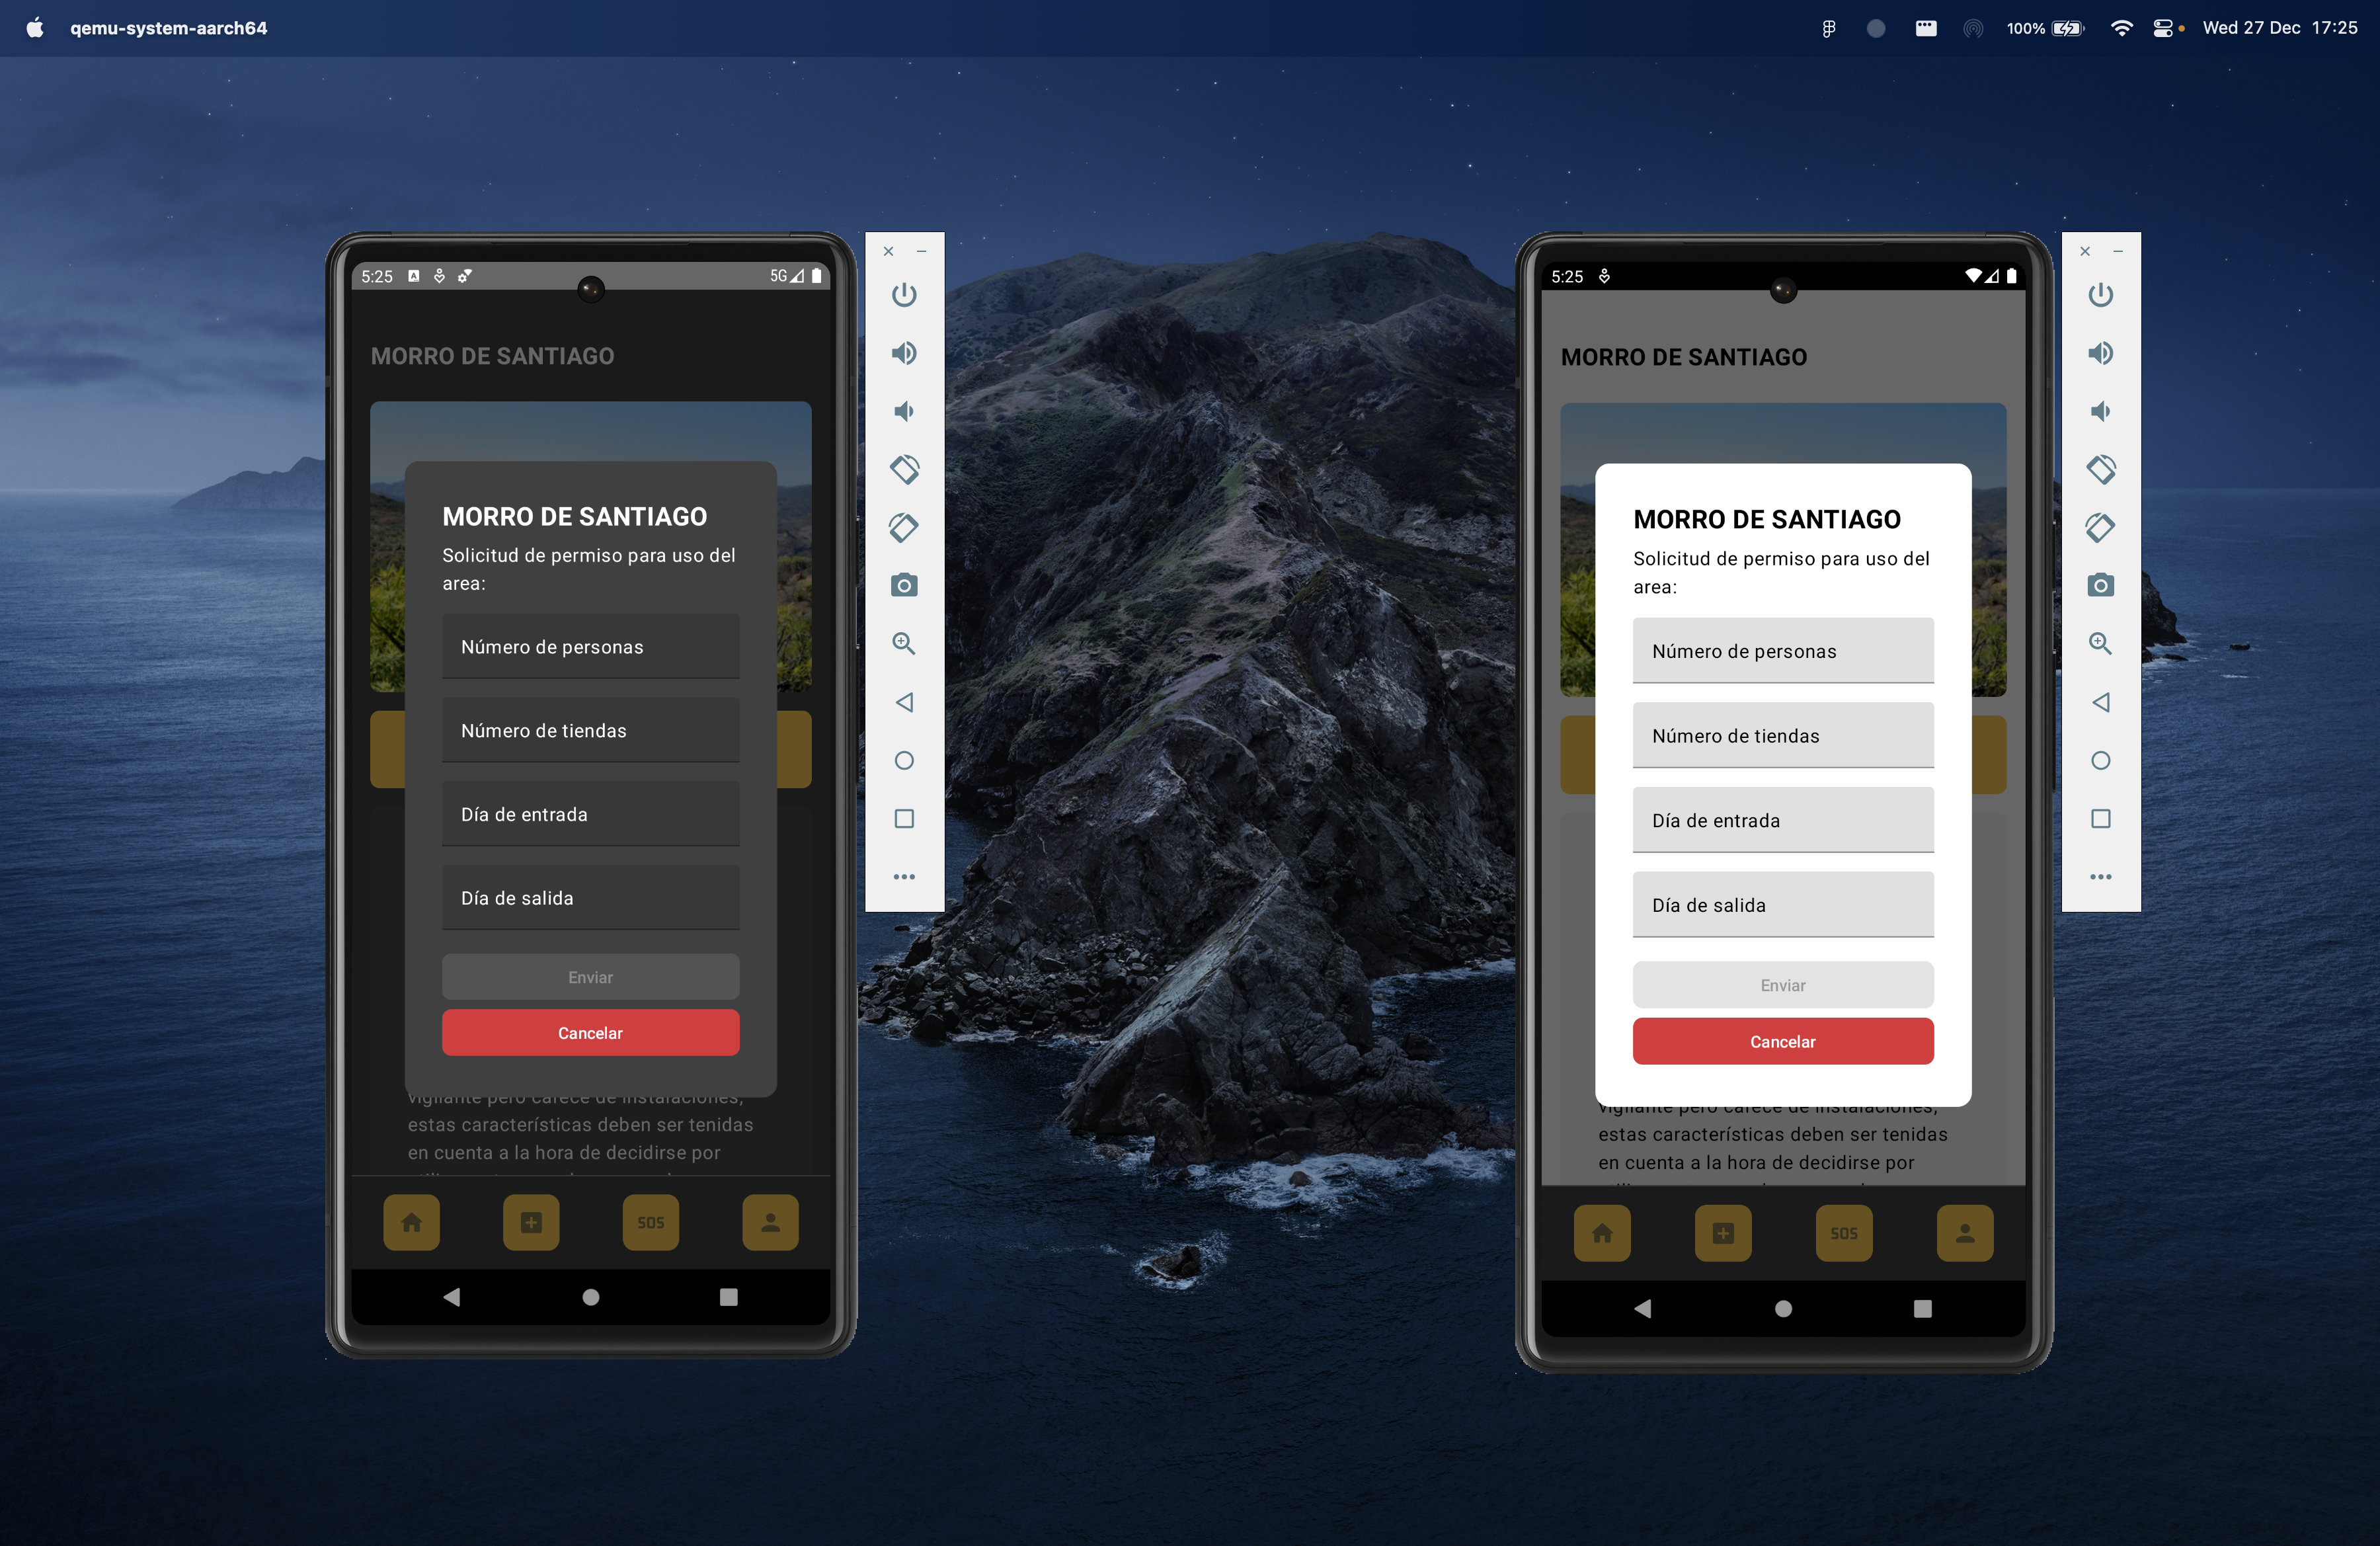
\includegraphics[scale=0.2]{area3.png}}
        \caption{Pantalla de area seleccionada, formulario de solicitud}
        \label{fig:area3}
    \end{figure}

    \begin{figure}[H]
        \centerline{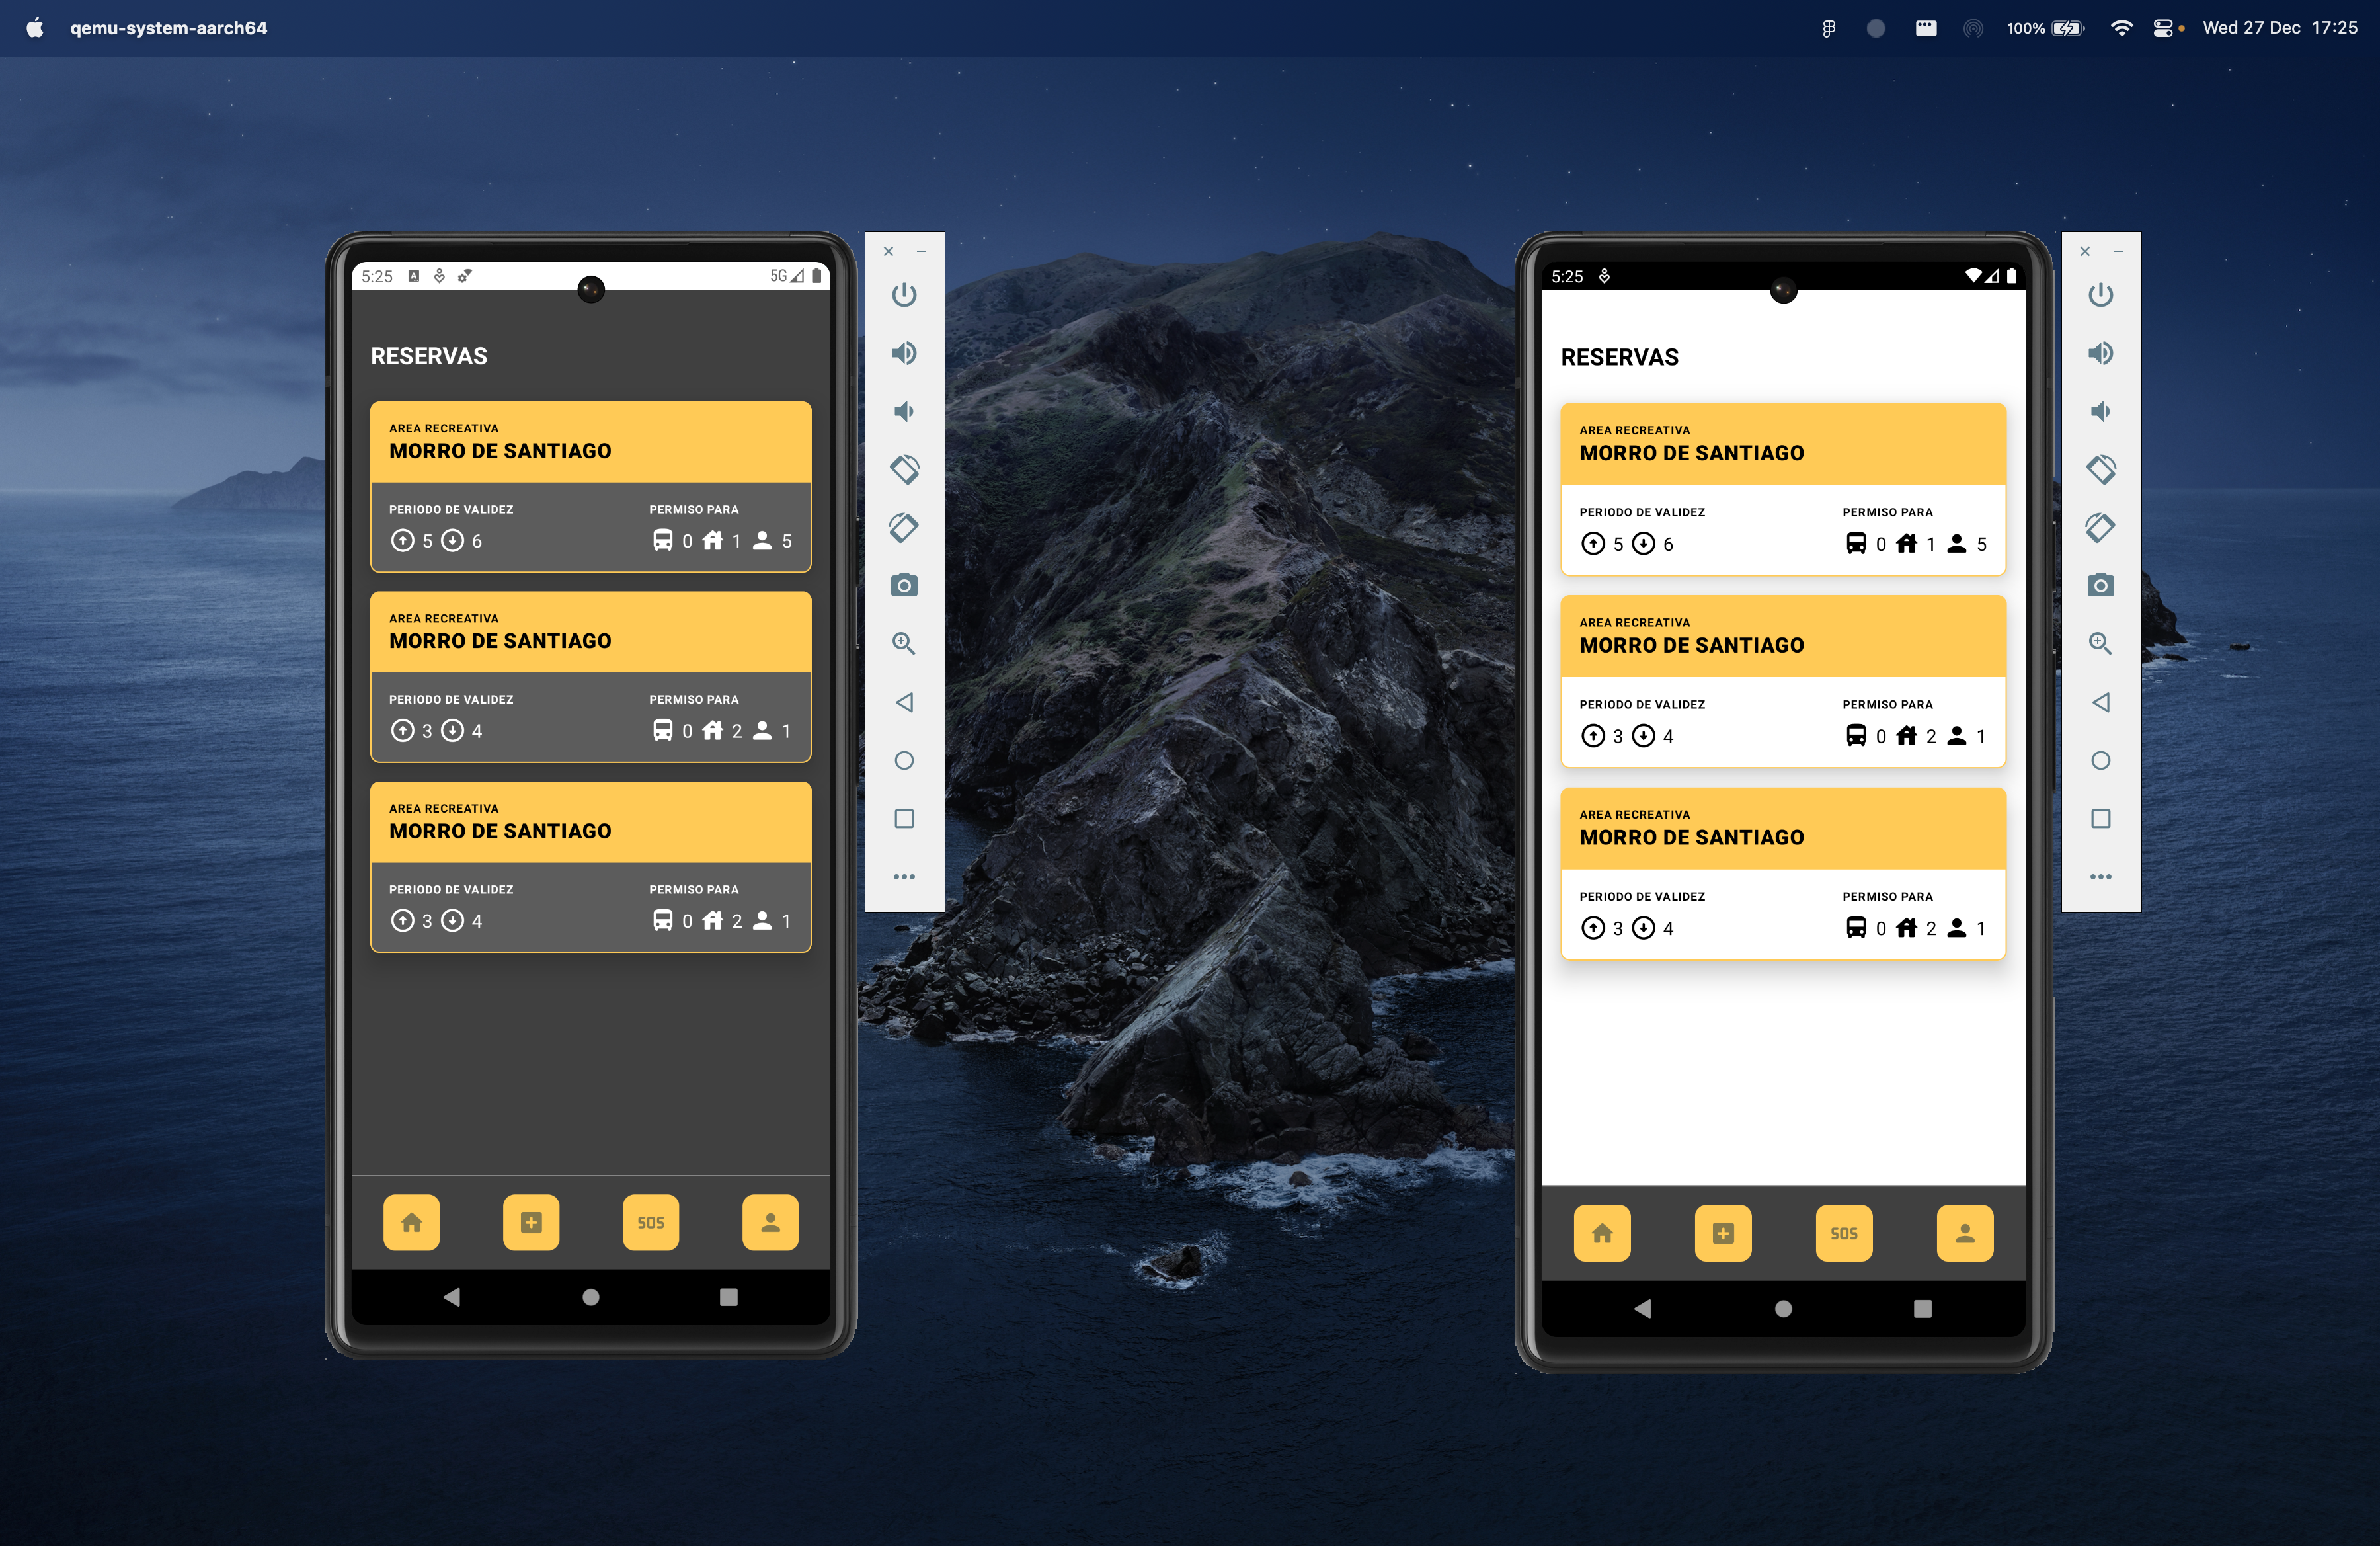
\includegraphics[scale=0.2]{book1.png}}
        \caption{Pantalla de solicitudes}
        \label{fig:book1}
    \end{figure}

    \begin{figure}[H]
        \centerline{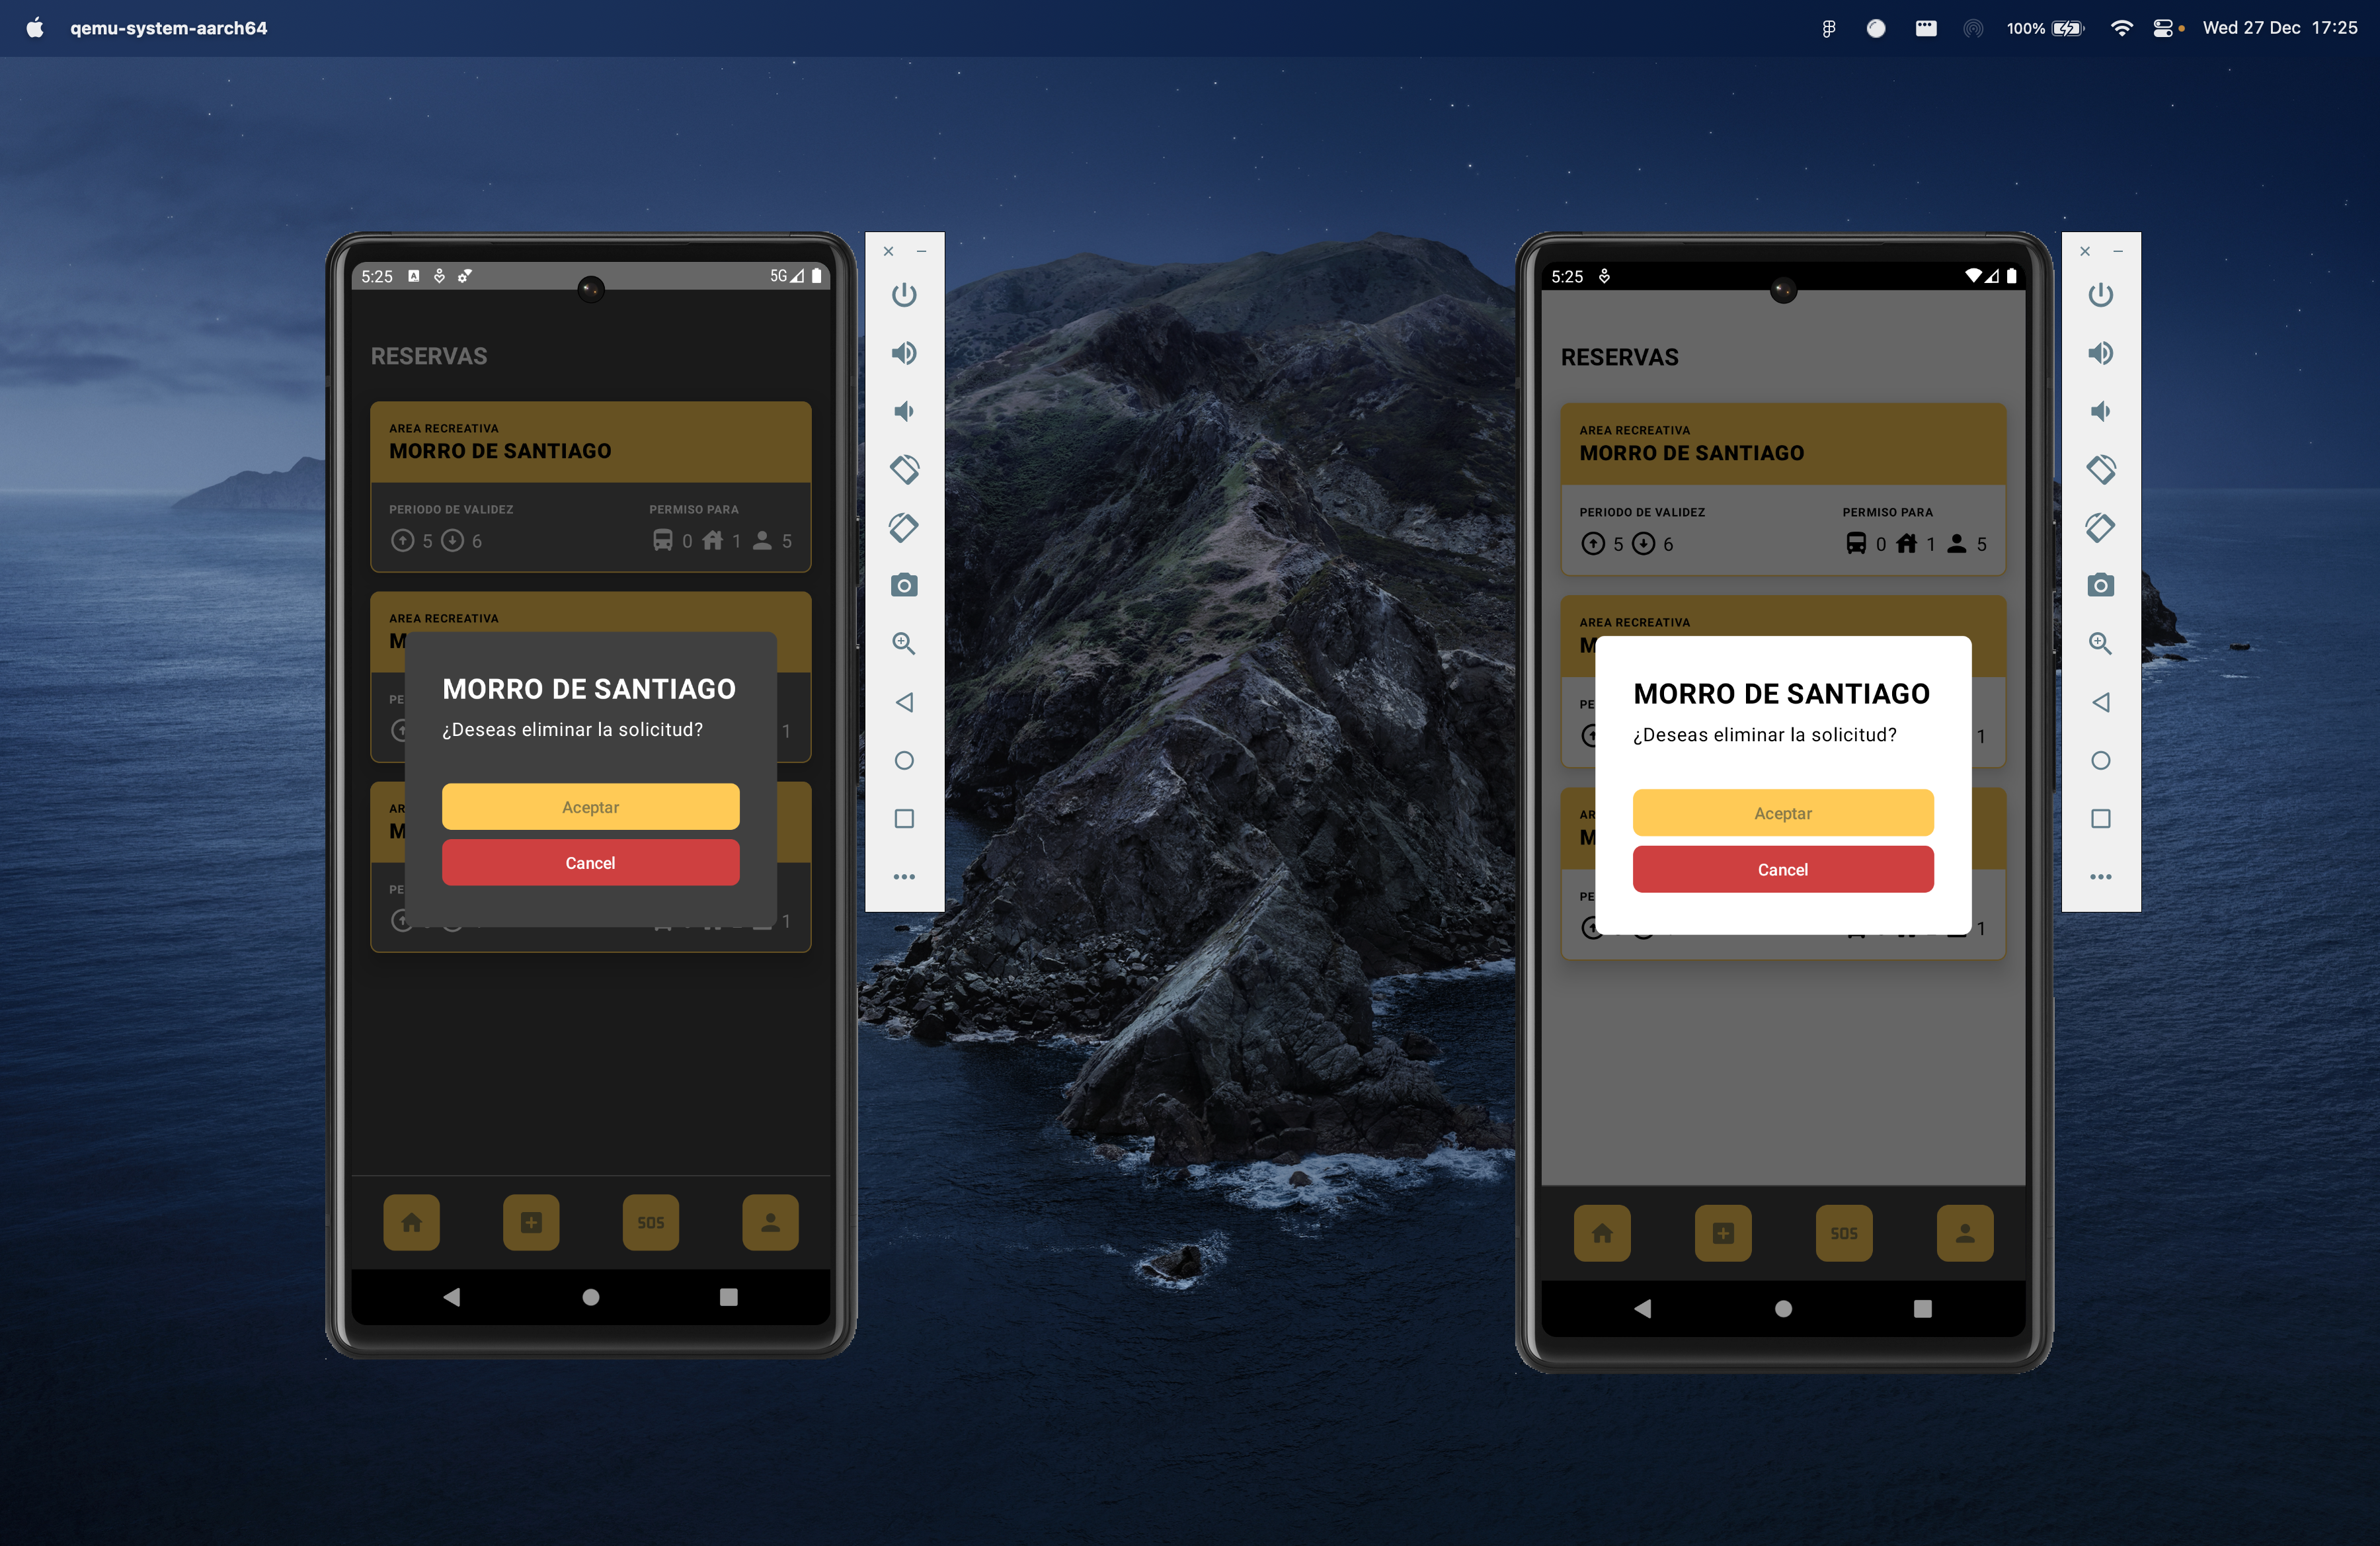
\includegraphics[scale=0.2]{book2.png}}
        \caption{Pantalla de solicitudes, formulario de eliminación}
        \label{fig:book2}
    \end{figure}

    \begin{figure}[H]
        \centerline{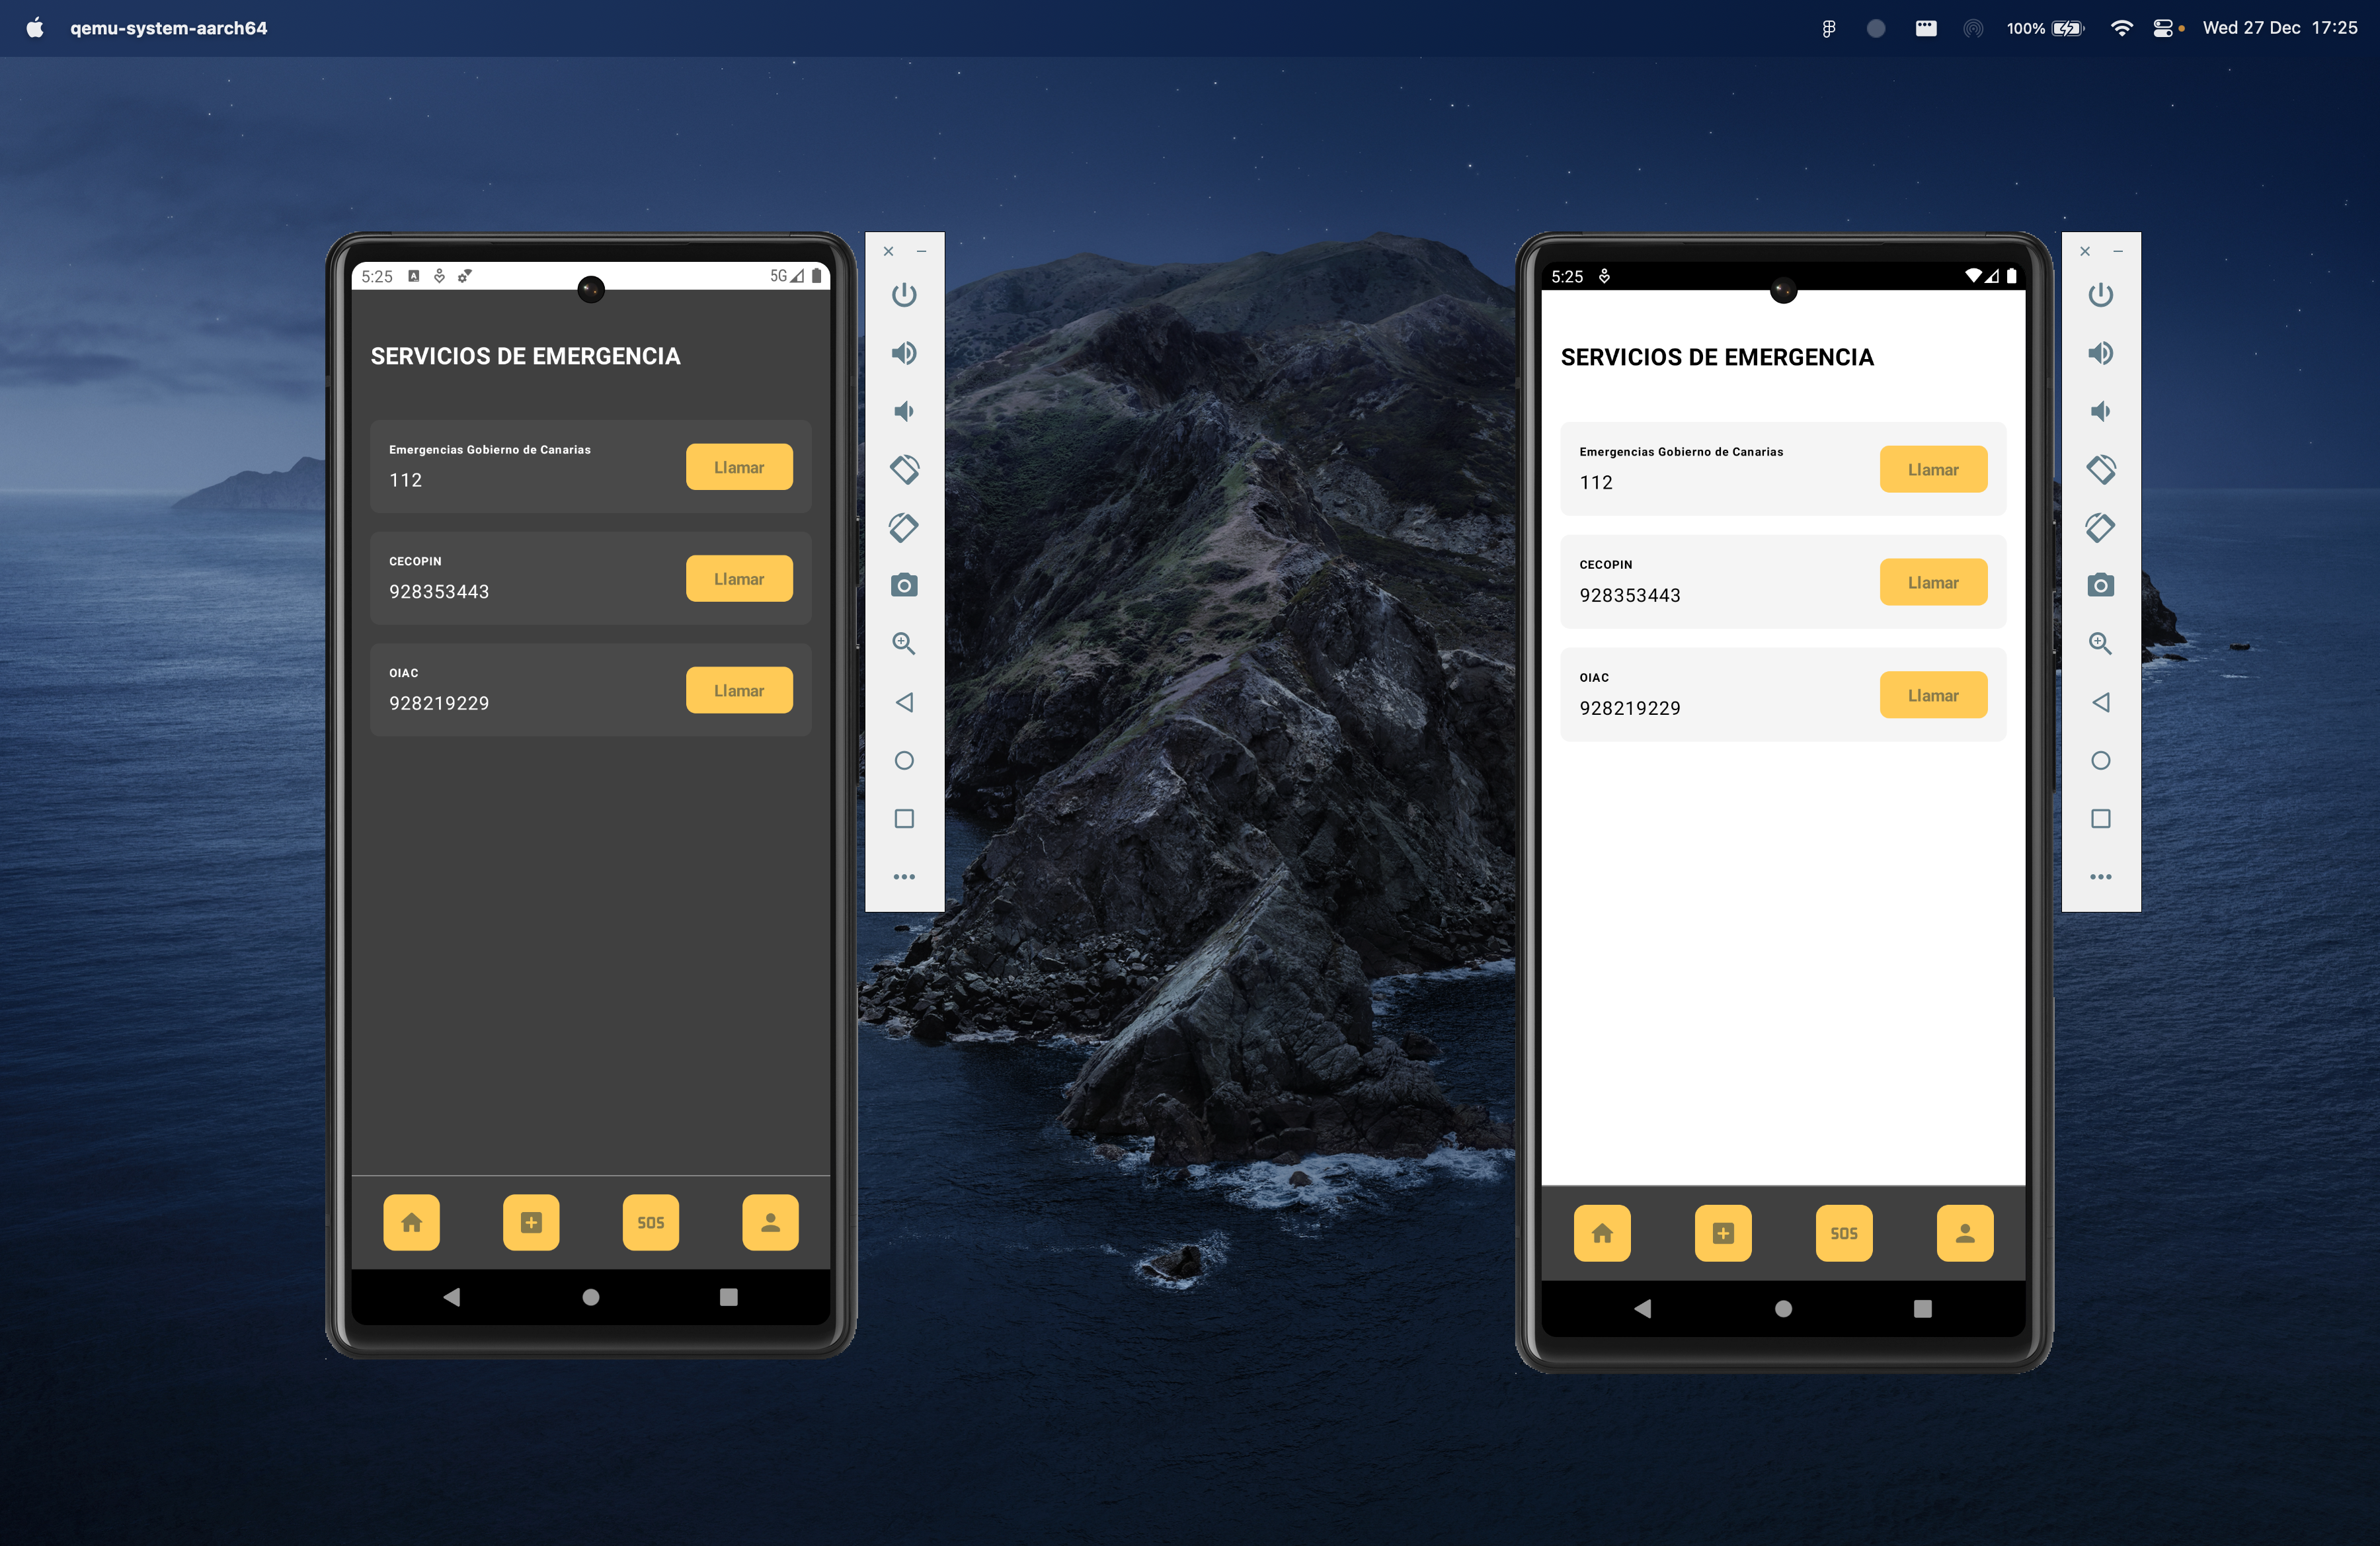
\includegraphics[scale=0.2]{emergencies.png}}
        \caption{Pantalla de emergencia}
        \label{fig:emergencies}
    \end{figure}

    \begin{figure}[H]
        \centerline{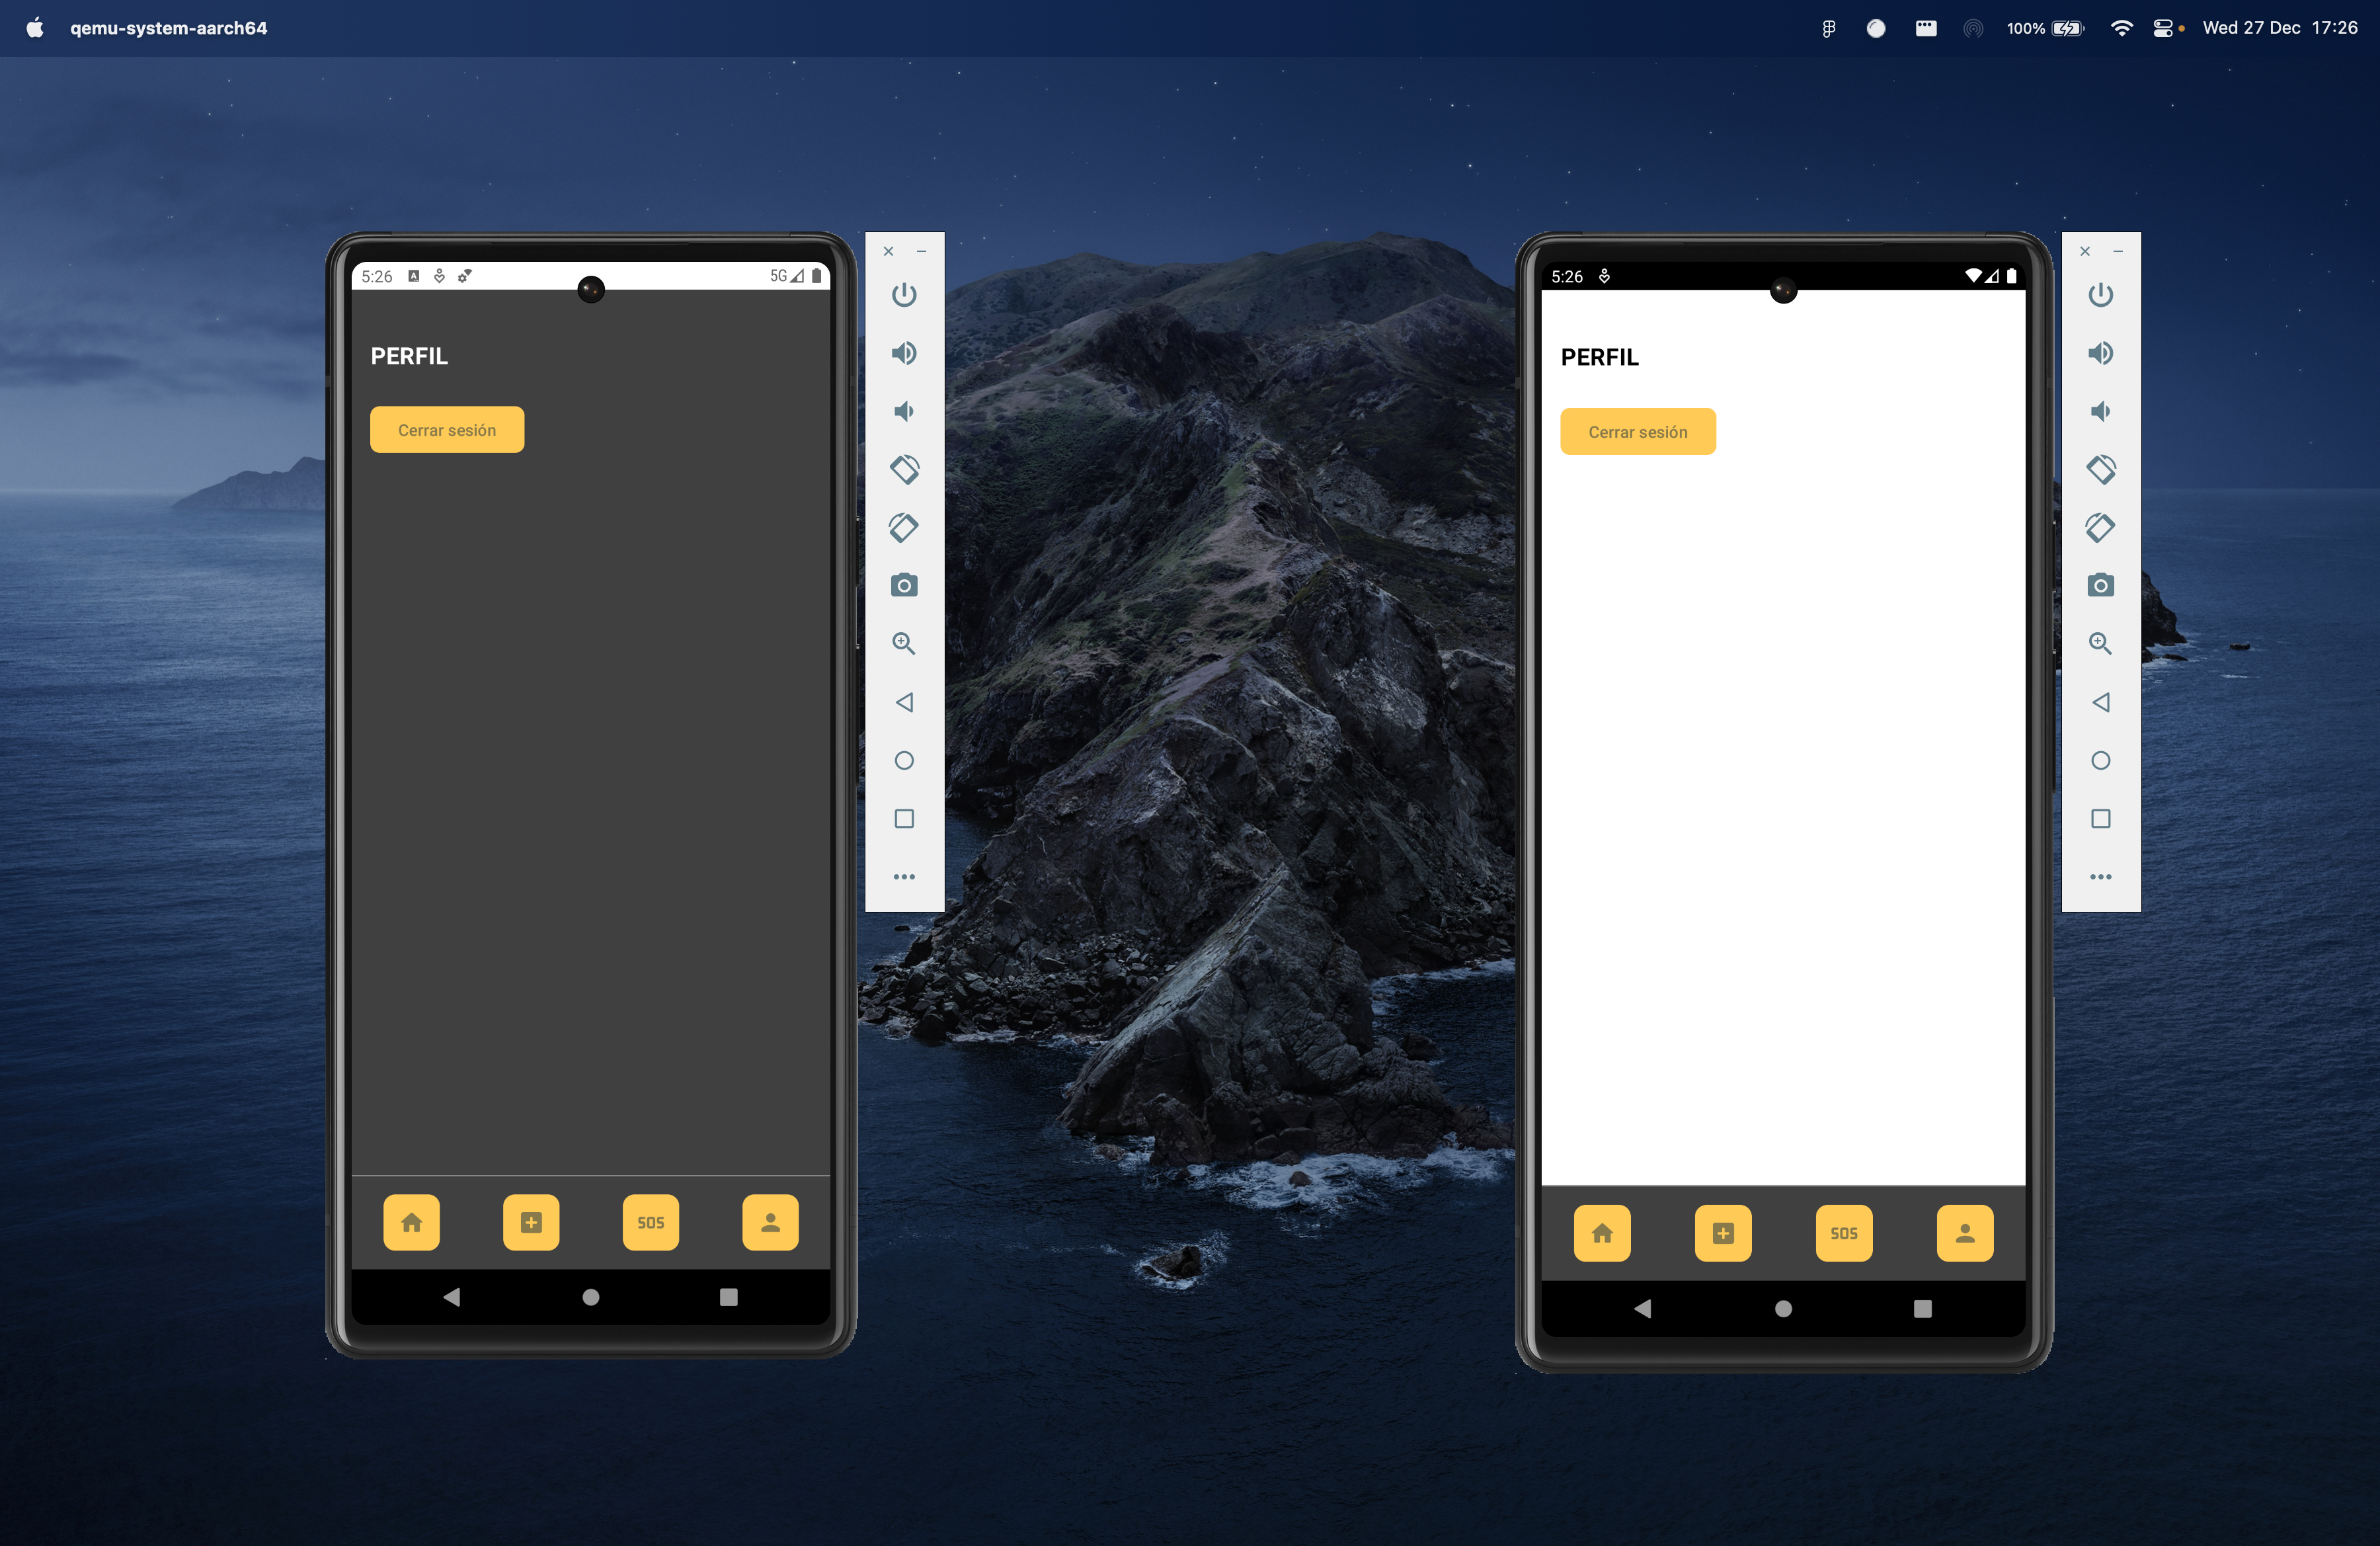
\includegraphics[scale=0.2]{profile.png}}
        \caption{Pantalla de perfil}
        \label{fig:profile}
    \end{figure}
\end{document}